\documentclass{article}

\usepackage{booktabs}
\usepackage{microtype}
\usepackage{pgfplots}
\usepackage{amsmath}

\title{Mandatory Assignment 2 - Neural Nets}
\author{Kris-Mikael Krister (krismikk)\\\texttt{krismikael@protonmail.com}}
\date{\today}

\begin{document}

\maketitle

\section*{Implementation}

The number of inputs and outputs to the neural network is fixed, and the network is constraint to include one hidden layer. These are constrained hyperparameters for the neural network that won't change.

The network is trained using a subset of the total available data, called \emph{training data}. Another subset, called \emph{validation data}, is used to avoid overfitting the model to the training data. A third subset, called \emph{test data}, is used to verify how well the algorithm performs. By using a separate subset for test data one can more accurately measure how generalized the trained model is. One full run of the algorithm is summarized as the following steps.

\begin{itemize}
    \item The available data is separated into training data, test data and validation data. The ratio is set to $50\%$, $25\%$ and $25\%$ of the total data respectively.
    \item One hidden layer is configured.
    \item Weights are randomly generated.
    \item The network is trained and updates the weights a fixed number of iterations, set to $100$.
    \item After training, the model is verified using the validation data. An error value is calculated.
    \item Training/validation repeat until the error value stops decreasing. This process is called \emph{earlystopping}.
    \item The model is tested using the test data and a confusion matrix is generated. The confusion matrix includes the percentage of correct values.
\end{itemize}

\noindent The amount of nodes/neurons in the hidden layer is a hyperparameter just as the number of input/ouput nodes. The amount can, in contrast to the other fixed hyperparameters, be tuned to generate the best model. I chose to find the number by trial and error.

Initial weights are randomly generated in the algorithm, so the algorithm should run multiple times and the \emph{score} for each hidden node is calculated from the mean of the results. The graph below shows the percentage of correct values for each tenth hidden node from $1 - 300$ ($n$ where $(n + 1) \mod{10} = 0$). The mean is calculated from 5 runs, where one full run is explained in the itemized list.\\\\

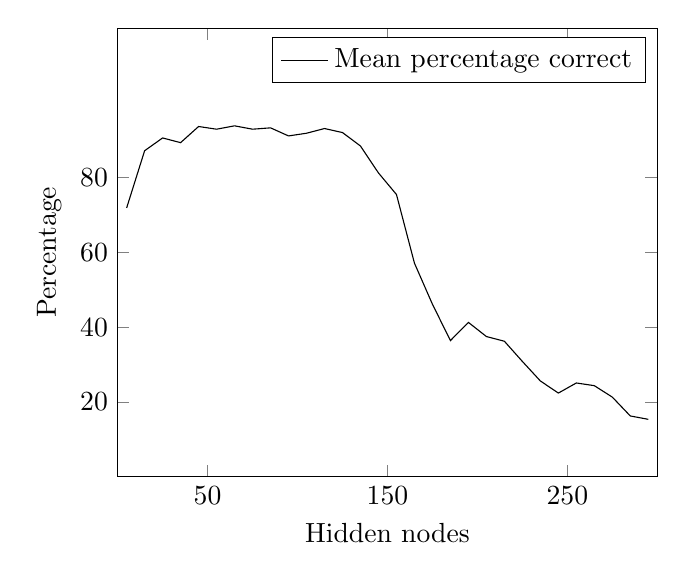
\begin{tikzpicture}
\begin{axis}[
    xlabel={Hidden nodes},
    ylabel={Percentage},
    xmin=0, xmax=300,
    ymin=0, ymax=120,
    xtick={50,150,250},
    ytick={20,40,60,80}
]
\addplot[
]
coordinates {
    (5,71.8918918919)(15,87.2072072072)(25,90.6306306306)(35,89.3693693694)(45,93.6936936937)(55,92.972972973)(65,93.8738738739)(75,92.972972973)(85,93.3333333333)(95,91.1711711712)(105,91.8918918919)(115,93.1531531532)(125,92.0720720721)(135,88.4684684685)(145,81.2612612613)(155,75.4954954955)(165,57.1171171171)(175,46.1261261261)(185,36.3963963964)(195,41.2612612613)(205,37.4774774775)(215,36.2162162162)(225,30.8108108108)(235,25.5855855856)(245,22.3423423423)(255,25.045045045)(265,24.3243243243)(275,21.2612612613)(285,16.2162162162)(295,15.3153153153)
};
\legend{Mean percentage correct}
\end{axis}
\end{tikzpicture}

\noindent The results indicate the value converge to a maximum for just a few hidden nodes. Another interesting find is that around 150 hidden nodes the results drops significantly, which could mean the network ends up having too many variations for the problem. For these two reasons, I will go more into detail for the nodes 5 \ndash 30. Each of the nodes are verified, and the number of runs for each node is increased from 5 to 50. The mean is calculated and shown in the graph below.\\\\

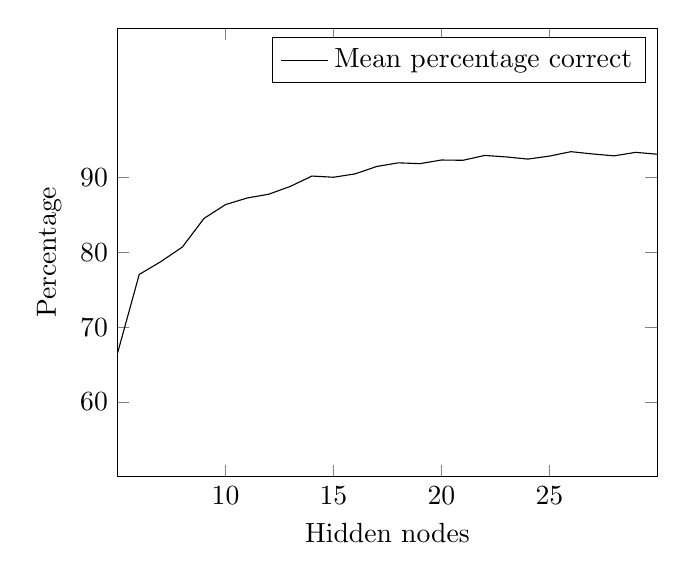
\begin{tikzpicture}
\begin{axis}[
    xlabel={Hidden nodes},
    ylabel={Percentage},
    xmin=5, xmax=30,
    ymin=50, ymax=110,
    xtick={10,15,20,25},
    ytick={60,70,80,90}
]
\addplot[
]
coordinates {
    (5,66.5585585586)(6,77.045045045)(7,78.7567567568)(8,80.7207207207)(9,84.5405405405)(10,86.3963963964)(11,87.2792792793)(12,87.7837837838)(13,88.8288288288)(14,90.2162162162)(15,90.0540540541)(16,90.5045045045)(17,91.4954954955)(18,91.981981982)(19,91.8738738739)(20,92.3603603604)(21,92.3243243243)(22,92.972972973)(23,92.7747747748)(24,92.4864864865)(25,92.8828828829)(26,93.4774774775)(27,93.1711711712)(28,92.9189189189)(29,93.3873873874)(30,93.1351351351)
};
\legend{Mean percentage correct}
\end{axis}
\end{tikzpicture}

\noindent For 14 hidden nodes, the mean percentage correct is $90.2\%$. The number converges to $\approx 92\%$ for 18 nodes. However, adding nodes to the network also increase the running for the algorithm. 14 nodes are therefore sufficient for this network to classify well. The table below shows results for even-numbered nodes starting from 12.

\begin{center}
\begin{tabular}{cc}
\toprule
Hidden nodes & Mean percentage correct \\
\midrule
12 & $87.8$\\
14 & $90.2$\\
16 & $90.5$\\
18 & $92.0$\\
20 & $92.3$\\
22 & $92.3$\\
22 & $92.5$\\
24 & $92.5$\\
26 & $93.5$\\
28 & $92.9$\\
30 & $93.1$\\
\bottomrule
\end{tabular}
\end{center}

\section*{Confusion Matrix}

\noindent The confusion matrix for 14 nodes is shown below with $91.9\%$ correct classifications. Values on the diagonal represents number of correctly classified instances, and values outside the diagonal are incorrectly classified instances. For example, Class 1 (the first row in the matrix) classifies incorrectly three times to Class 4, 5 and 6, respectively. Class 5 (the fifth row) is incorrectly classified two times for being Class 4.

\begin{itemize}
    \item Class 1 incorrectly classified to Class 4, 5 and 6.
    \item Class 5 incorrectly classified to Class 4.
    \item Class 7 incorrectly classified to Class 3 and 6.
    \item Class 8 incorrectly classified to Class 1 and 4.
\end{itemize}

\noindent Based on the confusion matrix, it seems like the network has some issues with correctly classifying Class 1, 4 and 6.

\begin{center}
\begin{verbatim}
[  8.   0.   0.   1.   1.   1.   0.   0.]
[  0.  17.   0.   0.   0.   0.   0.   0.]
[  0.   0.  19.   0.   0.   0.   0.   0.]
[  0.   0.   0.  12.   0.   0.   0.   0.]
[  0.   0.   0.   2.   9.   0.   0.   0.]
[  0.   0.   0.   0.   0.  11.   0.   0.]
[  0.   0.   1.   0.   0.   1.  12.   0.]
[  1.   0.   0.   1.   0.   0.   0.  14.]
\end{verbatim}
\end{center}

\section*{K-Fold Cross Validation}

A problem with splitting the available data into three subsets is that some of the data is not used for training. By splitting the available data into $K$ \emph{folds} and running the algorithm $K$ times with different data, we're able to train and validate the data on the whole dataset. The model we choose in the end will be the one that generates the highest amount of correct classifications (the one with the lowest error value). Number of hidden nodes is set to 14. The data is split into training, testing and validation as already explained, and the ratio between the splits are unchanged. The difference is that the content of the subsets differ in each fold.

The table below shows data for 6 different fold sizes. Note that data in each row are from \emph{K single runs}, where $K$ is the amount of folds. This is in contrast to the previous implementation where the data is calculated from the mean value of $n$ runs, where $n$ is a fixed number.

\begin{center}
\begin{tabular}{cccc}
\toprule
Num folds ($K$) & Max & Mean & Std.dev. \\
\midrule
1 & $80.4\%$ & $80.4\%$ & $0.0$\\
4 & $86.6\%$ & $85.3\%$ & $0.8$\\
7 & $90.2\%$ & $86.5\%$ & $3.2$\\
10 & $93.8\%$ & $86.0\%$ & $8.5$\\
20 & $96.4\%$ & $91.7\%$ & $2.8$\\
30 & $89.3\%$ & $84.9\%$ & $2.7$\\
\bottomrule
\end{tabular}
\end{center}

\noindent The results above indicate that the quality of the model can be increased by using a multi-fold cross validation. For example, when using 4 folds, the mean percentage of correct values increase from $80.4\%$ to $85.3\%$. When using 20 folds, the best model achieves $96.4\%$ correct values. That is currently the best value seen with this implementation. However, due to the stochastic nature of the algorithm it's too early to conclude whether that model is guaranteed to be superior in all cases.

Two confusion matrices for the K-Fold Cross Validation are shown in the next section.

\section*{Running The Program}

The entry point for the program is \textit{movements.py}, and can run in three different ways.

\subsection*{Basic Run}

The following command will train the network with 14 hidden nodes and print a confusion matrix together with percentage correct values.

\begin{verbatim}
$ python movements.py

Confusion matrix:
[[  8.   0.   0.   0.   1.   0.   0.   0.]
 [  0.  19.   0.   0.   0.   0.   0.   4.]
 [  0.   0.   9.   0.   0.   0.   1.   1.]
 [  0.   0.   0.  10.   2.   0.   0.   0.]
 [  0.   0.   0.   1.  21.   0.   0.   0.]
 [  0.   1.   0.   0.   0.   5.   2.   0.]
 [  0.   0.   0.   1.   0.   4.   8.   0.]
 [  0.   0.   0.   0.   0.   0.   0.  13.]]
Percentage correct:
83.7837837838
\end{verbatim}

\subsection*{Different Number of Hidden Nodes}

The following command will train the network 50 times and print the mean error for these runs. Number of hidden nodes spans 5 \ndash 30.

\begin{verbatim}
$ python movements.py mean

number_of_hidden_nodes,mean_percentage_correct
5,65.027027027
6,73.9459459459
7,77.1171171171
8,78.2882882883
9,81.5315315315
10,83.7477477477
11,84.4864864865
12,85.4594594595
13,85.6576576577
14,86.990990991
15,87.7657657658
16,88.1981981982
17,89.8918918919
18,90.1621621622
19,90.2162162162
20,89.5135135135
21,90.8648648649
22,90.8108108108
23,91.3693693694
24,91.7297297297
25,91.5135135135
26,91.6396396396
27,92.3423423423
28,91.6576576577
29,92.3603603604
30,92.3243243243
\end{verbatim}

\subsection*{K-Fold Cross Validation}

The following command will train the network using $K$-folds and print the percentage correct values together with confusion matrices for all of the folds. Max percentage correct, standard deviation and the average percentage correct over the folds are printed below the last fold.

\begin{verbatim}
$ python movements.py kfold 10

Confusion matrix:Fold 0
Confusion matrix:
[[ 16.   0.   0.   0.   0.   0.   0.   0.]
 [  0.  13.   0.   0.   0.   1.   1.   0.]
 [  0.   0.   8.   1.   0.   0.   0.   1.]
 [  0.   0.   0.  13.   0.   0.   1.   1.]
 [  2.   0.   0.   1.  14.   0.   1.   0.]
 [  0.   1.   0.   0.   0.   8.   5.   0.]
 [  0.   0.   0.   0.   0.   0.  11.   0.]
 [  0.   0.   1.   0.   0.   0.   0.  12.]]
Percentage correct:
84.8214285714

""" 8 folds are hidden for brevity """

Fold 9
Confusion matrix:
[[ 16.   0.   0.   0.   0.   0.   0.   1.]
 [  0.  13.   0.   0.   0.   0.   1.   0.]
 [  0.   0.   8.   0.   0.   0.   0.   0.]
 [  0.   0.   0.  13.   0.   0.   0.   0.]
 [  2.   0.   0.   1.  14.   0.   0.   0.]
 [  0.   1.   0.   0.   0.   9.   3.   0.]
 [  0.   0.   0.   0.   0.   0.  15.   0.]
 [  0.   0.   1.   1.   0.   0.   0.  13.]]
Percentage correct:
90.1785714286

max 93.75
std 5.10492584247
avg 84.9107142857
\end{verbatim}

\end{document}
